\documentclass[10pt]{article}
\usepackage[margin=0.65in]{geometry}
\usepackage{graphicx,hyperref,parskip,amssymb}
\hypersetup{colorlinks=true,urlcolor=blue}
\begin{document}
\begin{center}\Large Bounded GPU continuation: preparation record\\
\normalsize Audit items 7 and 13; 18 October 2026\end{center}
\textbf{Prepared; no remote GPU result yet.} One dedicated RunPod GPU with
a two-hour lifetime is authorized. Root owns provisioning, credential
handling, evidence retrieval and deletion. Existing resources and shared
campaign stores are untouched.

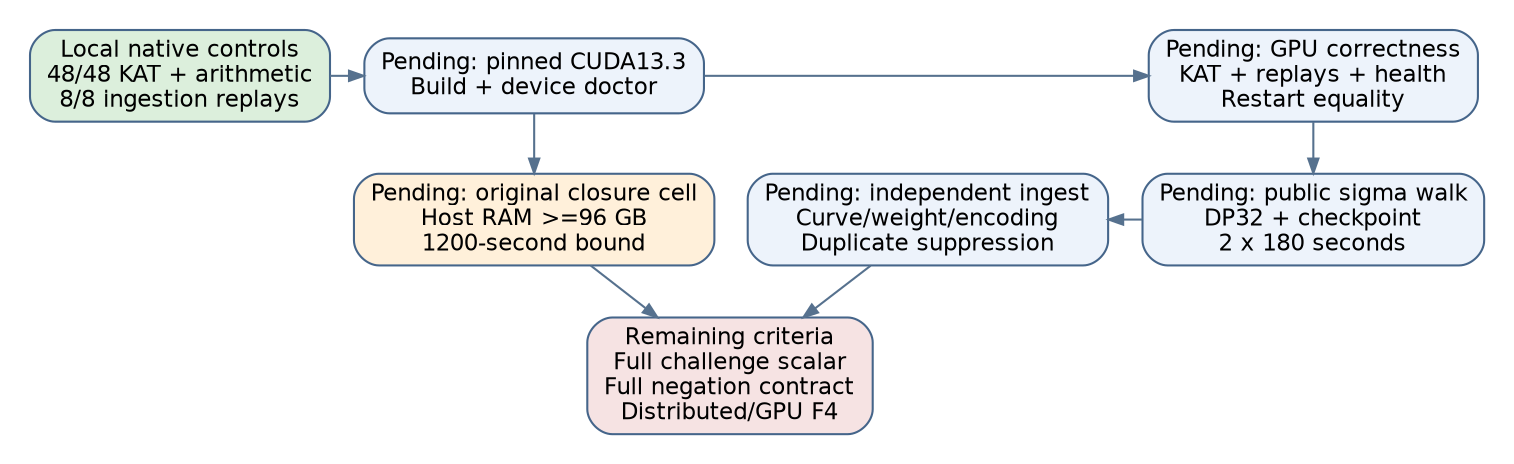
\includegraphics[width=\linewidth]{run-flow.png}

The native ECC2K-130 sigma client is pinned to cryptanalysis revision
\texttt{0ea8931d21d567f83de47c30bdaac0585f479c11}; 39 required source files
are hashed in \texttt{source/ecc.sha256}. It uses the public challenge P/Q
on $y^2+xy=x^3+1$ over $\mathbb F_{2^{131}}$, in the exact permuted type-II
normal basis named by its source. The subgroup order is
\[680564733841876926932320129493409985129.\]
A polynomial-basis registry ID
does not stand in for the native normal-basis representation.

\textbf{Completed CPU correctness controls.} Host sigma tests passed
2862 checks including 48/48 campaign known answers. Native carry-less and
portable software controls passed 28,633 and 28,639 checks, respectively.
The new native ingestion checker accepted eight independently generated
positive-length reports and re-walked all eight on the golden model. A
changed coordinate was rejected. The first fixture's zero-length trail was
rejected and its failure retained. These are correctness checks, not GPU
coverage or timing evidence.

\textbf{Prospective remote sequence.} The launcher requires the pinned
CUDA13.3.73 compiler, compatible device/runtime, native KAT, three GPU
golden-model replays, a health test and identical record multisets across a
checkpoint restart. It then collects two 180-second sigma slices at DP
weight32 with public P/Q, max-iters $2^{32}$ and periodic checkpoints.
Graceful SIGTERM ends each slice; the second resumes the first checkpoint.
Three throughput samples are diagnostics, with no speedup or host-isolation
claim. Every command preserves stdout, stderr, exit and resource records.

The independent native ingester checks every retained full report against
the golden model's curve equation, weight, seed namespace and DP32 orbit
encoding. It replays only bounded short trails: long challenge trails
remain explicitly unreplayed. Native merge and repeated ingestion retain
duplicate, collision and malformed counts. Run53181 is quarantined: a
global campaign lease is not claimed, and no shared-store upload occurs.
A collision is not scalar recovery; challenge completion requires an
independently verified discrete logarithm.

\textbf{Other original criteria.} H-RHO-bc6ea6 / EXP-RHO-60da4f already has
substantial trials. Copied native source and implementation notes disclose
its affine/Jacobian deviation, heavy censoring and limited baseline gates.
A four-arm L32 replay here is instrument continuation only; the sigma
client cannot close that prime-field contract. The native closure probe has
separate input, runtime and memory gates and a1200-second limit; a
fixed-degree reducer cannot substitute for solving degree D.

\textbf{Evidence and limits.} See the source-linked \texttt{README.md},
\texttt{PROTOCOL.md}, native launch/checker, source manifests and
\texttt{local\_checks/}. Remote outputs are pending. Existing IC leaderboard
and ECC2K campaign GPU/rate figures remain historical: no new remote datum
exists to change them. Full challenge completion, the full negation
contract, and distributed/GPU F4 remain open. No commits or pushes were
made by this workstream.
\end{document}
